%% bare_conf.tex
%% V1.4b
%% 2015/08/26
%% by Michael Shell
%% See:
%% http://www.michaelshell.org/
%% for current contact information.
%%
%% This is a skeleton file demonstrating the use of IEEEtran.cls
%% (requires IEEEtran.cls version 1.8b or later) with an IEEE
%% conference paper.
%%
%% Support sites:
%% http://www.michaelshell.org/tex/ieeetran/
%% http://www.ctan.org/pkg/ieeetran
%% and
%% http://www.ieee.org/

%%*************************************************************************
%% Legal Notice:
%% This code is offered as-is without any warranty either expressed or
%% implied; without even the implied warranty of MERCHANTABILITY or
%% FITNESS FOR A PARTICULAR PURPOSE! 
%% User assumes all risk.
%% In no event shall the IEEE or any contributor to this code be liable for
%% any damages or losses, including, but not limited to, incidental,
%% consequential, or any other damages, resulting from the use or misuse
%% of any information contained here.
%%
%% All comments are the opinions of their respective authors and are not
%% necessarily endorsed by the IEEE.
%%
%% This work is distributed under the LaTeX Project Public License (LPPL)
%% ( http://www.latex-project.org/ ) version 1.3, and may be freely used,
%% distributed and modified. A copy of the LPPL, version 1.3, is included
%% in the base LaTeX documentation of all distributions of LaTeX released
%% 2003/12/01 or later.
%% Retain all contribution notices and credits.
%% ** Modified files should be clearly indicated as such, including  **
%% ** renaming them and changing author support contact information. **
%%*************************************************************************


% *** Authors should verify (and, if needed, correct) their LaTeX system  ***
% *** with the testflow diagnostic prior to trusting their LaTeX platform ***
% *** with production work. The IEEE's font choices and paper sizes can   ***
% *** trigger bugs that do not appear when using other class files.       ***                          ***
% The testflow support page is at:
% http://www.michaelshell.org/tex/testflow/



\documentclass[conference]{IEEEtran}

\usepackage{xcolor}
\usepackage{graphicx}
\usepackage{amsmath}
%\usepackage{hyperref}

% Some Computer Society conferences also require the compsoc mode option,
% but others use the standard conference format.
%
% If IEEEtran.cls has not been installed into the LaTeX system files,
% manually specify the path to it like:
% \documentclass[conference]{../sty/IEEEtran}





% Some very useful LaTeX packages include:
% (uncomment the ones you want to load)


% *** MISC UTILITY PACKAGES ***
%
%\usepackage{ifpdf}
% Heiko Oberdiek's ifpdf.sty is very useful if you need conditional
% compilation based on whether the output is pdf or dvi.
% usage:
% \ifpdf
%   % pdf code
% \else
%   % dvi code
% \fi
% The latest version of ifpdf.sty can be obtained from:
% http://www.ctan.org/pkg/ifpdf
% Also, note that IEEEtran.cls V1.7 and later provides a builtin
% \ifCLASSINFOpdf conditional that works the same way.
% When switching from latex to pdflatex and vice-versa, the compiler may
% have to be run twice to clear warning/error messages.






% *** CITATION PACKAGES ***
%
%\usepackage{cite}
% cite.sty was written by Donald Arseneau
% V1.6 and later of IEEEtran pre-defines the format of the cite.sty package
% \cite{} output to follow that of the IEEE. Loading the cite package will
% result in citation numbers being automatically sorted and properly
% "compressed/ranged". e.g., [1], [9], [2], [7], [5], [6] without using
% cite.sty will become [1], [2], [5]--[7], [9] using cite.sty. cite.sty's
% \cite will automatically add leading space, if needed. Use cite.sty's
% noadjust option (cite.sty V3.8 and later) if you want to turn this off
% such as if a citation ever needs to be enclosed in parenthesis.
% cite.sty is already installed on most LaTeX systems. Be sure and use
% version 5.0 (2009-03-20) and later if using hyperref.sty.
% The latest version can be obtained at:
% http://www.ctan.org/pkg/cite
% The documentation is contained in the cite.sty file itself.






% *** GRAPHICS RELATED PACKAGES ***
%
\ifCLASSINFOpdf
  % \usepackage[pdftex]{graphicx}
  % declare the path(s) where your graphic files are
  % \graphicspath{{../pdf/}{../jpeg/}}
  % and their extensions so you won't have to specify these with
  % every instance of \includegraphics
  % \DeclareGraphicsExtensions{.pdf,.jpeg,.png}
\else
  % or other class option (dvipsone, dvipdf, if not using dvips). graphicx
  % will default to the driver specified in the system graphics.cfg if no
  % driver is specified.
  % \usepackage[dvips]{graphicx}
  % declare the path(s) where your graphic files are
  % \graphicspath{{../eps/}}
  % and their extensions so you won't have to specify these with
  % every instance of \includegraphics
  % \DeclareGraphicsExtensions{.eps}
\fi
% graphicx was written by David Carlisle and Sebastian Rahtz. It is
% required if you want graphics, photos, etc. graphicx.sty is already
% installed on most LaTeX systems. The latest version and documentation
% can be obtained at: 
% http://www.ctan.org/pkg/graphicx
% Another good source of documentation is "Using Imported Graphics in
% LaTeX2e" by Keith Reckdahl which can be found at:
% http://www.ctan.org/pkg/epslatex
%
% latex, and pdflatex in dvi mode, support graphics in encapsulated
% postscript (.eps) format. pdflatex in pdf mode supports graphics
% in .pdf, .jpeg, .png and .mps (metapost) formats. Users should ensure
% that all non-photo figures use a vector format (.eps, .pdf, .mps) and
% not a bitmapped formats (.jpeg, .png). The IEEE frowns on bitmapped formats
% which can result in "jaggedy"/blurry rendering of lines and letters as
% well as large increases in file sizes.
%
% You can find documentation about the pdfTeX application at:
% http://www.tug.org/applications/pdftex





% *** MATH PACKAGES ***
%
%\usepackage{amsmath}
% A popular package from the American Mathematical Society that provides
% many useful and powerful commands for dealing with mathematics.
%
% Note that the amsmath package sets \interdisplaylinepenalty to 10000
% thus preventing page breaks from occurring within multiline equations. Use:
%\interdisplaylinepenalty=2500
% after loading amsmath to restore such page breaks as IEEEtran.cls normally
% does. amsmath.sty is already installed on most LaTeX systems. The latest
% version and documentation can be obtained at:
% http://www.ctan.org/pkg/amsmath





% *** SPECIALIZED LIST PACKAGES ***
%
%\usepackage{algorithmic}
% algorithmic.sty was written by Peter Williams and Rogerio Brito.
% This package provides an algorithmic environment fo describing algorithms.
% You can use the algorithmic environment in-text or within a figure
% environment to provide for a floating algorithm. Do NOT use the algorithm
% floating environment provided by algorithm.sty (by the same authors) or
% algorithm2e.sty (by Christophe Fiorio) as the IEEE does not use dedicated
% algorithm float types and packages that provide these will not provide
% correct IEEE style captions. The latest version and documentation of
% algorithmic.sty can be obtained at:
% http://www.ctan.org/pkg/algorithms
% Also of interest may be the (relatively newer and more customizable)
% algorithmicx.sty package by Szasz Janos:
% http://www.ctan.org/pkg/algorithmicx




% *** ALIGNMENT PACKAGES ***
%
%\usepackage{array}
% Frank Mittelbach's and David Carlisle's array.sty patches and improves
% the standard LaTeX2e array and tabular environments to provide better
% appearance and additional user controls. As the default LaTeX2e table
% generation code is lacking to the point of almost being broken with
% respect to the quality of the end results, all users are strongly
% advised to use an enhanced (at the very least that provided by array.sty)
% set of table tools. array.sty is already installed on most systems. The
% latest version and documentation can be obtained at:
% http://www.ctan.org/pkg/array


% IEEEtran contains the IEEEeqnarray family of commands that can be used to
% generate multiline equations as well as matrices, tables, etc., of high
% quality.




% *** SUBFIGURE PACKAGES ***
%\ifCLASSOPTIONcompsoc
%  \usepackage[caption=false,font=normalsize,labelfont=sf,textfont=sf]{subfig}
%\else
%  \usepackage[caption=false,font=footnotesize]{subfig}
%\fi
% subfig.sty, written by Steven Douglas Cochran, is the modern replacement
% for subfigure.sty, the latter of which is no longer maintained and is
% incompatible with some LaTeX packages including fixltx2e. However,
% subfig.sty requires and automatically loads Axel Sommerfeldt's caption.sty
% which will override IEEEtran.cls' handling of captions and this will result
% in non-IEEE style figure/table captions. To prevent this problem, be sure
% and invoke subfig.sty's "caption=false" package option (available since
% subfig.sty version 1.3, 2005/06/28) as this is will preserve IEEEtran.cls
% handling of captions.
% Note that the Computer Society format requires a larger sans serif font
% than the serif footnote size font used in traditional IEEE formatting
% and thus the need to invoke different subfig.sty package options depending
% on whether compsoc mode has been enabled.
%
% The latest version and documentation of subfig.sty can be obtained at:
% http://www.ctan.org/pkg/subfig




% *** FLOAT PACKAGES ***
%
%\usepackage{fixltx2e}
% fixltx2e, the successor to the earlier fix2col.sty, was written by
% Frank Mittelbach and David Carlisle. This package corrects a few problems
% in the LaTeX2e kernel, the most notable of which is that in current
% LaTeX2e releases, the ordering of single and double column floats is not
% guaranteed to be preserved. Thus, an unpatched LaTeX2e can allow a
% single column figure to be placed prior to an earlier double column
% figure.
% Be aware that LaTeX2e kernels dated 2015 and later have fixltx2e.sty's
% corrections already built into the system in which case a warning will
% be issued if an attempt is made to load fixltx2e.sty as it is no longer
% needed.
% The latest version and documentation can be found at:
% http://www.ctan.org/pkg/fixltx2e


%\usepackage{stfloats}
% stfloats.sty was written by Sigitas Tolusis. This package gives LaTeX2e
% the ability to do double column floats at the bottom of the page as well
% as the top. (e.g., "\begin{figure*}[!b]" is not normally possible in
% LaTeX2e). It also provides a command:
%\fnbelowfloat
% to enable the placement of footnotes below bottom floats (the standard
% LaTeX2e kernel puts them above bottom floats). This is an invasive package
% which rewrites many portions of the LaTeX2e float routines. It may not work
% with other packages that modify the LaTeX2e float routines. The latest
% version and documentation can be obtained at:
% http://www.ctan.org/pkg/stfloats
% Do not use the stfloats baselinefloat ability as the IEEE does not allow
% \baselineskip to stretch. Authors submitting work to the IEEE should note
% that the IEEE rarely uses double column equations and that authors should try
% to avoid such use. Do not be tempted to use the cuted.sty or midfloat.sty
% packages (also by Sigitas Tolusis) as the IEEE does not format its papers in
% such ways.
% Do not attempt to use stfloats with fixltx2e as they are incompatible.
% Instead, use Morten Hogholm'a dblfloatfix which combines the features
% of both fixltx2e and stfloats:
%
% \usepackage{dblfloatfix}
% The latest version can be found at:
% http://www.ctan.org/pkg/dblfloatfix




% *** PDF, URL AND HYPERLINK PACKAGES ***
%
%\usepackage{url}
% url.sty was written by Donald Arseneau. It provides better support for
% handling and breaking URLs. url.sty is already installed on most LaTeX
% systems. The latest version and documentation can be obtained at:
% http://www.ctan.org/pkg/url
% Basically, \url{my_url_here}.




% *** Do not adjust lengths that control margins, column widths, etc. ***
% *** Do not use packages that alter fonts (such as pslatex).         ***
% There should be no need to do such things with IEEEtran.cls V1.6 and later.
% (Unless specifically asked to do so by the journal or conference you plan
% to submit to, of course. )


% correct bad hyphenation here
\hyphenation{op-tical net-works semi-conduc-tor}


\begin{document}
%
% paper title
% Titles are generally capitalized except for words such as a, an, and, as,
% at, but, by, for, in, nor, of, on, or, the, to and up, which are usually
% not capitalized unless they are the first or last word of the title.
% Linebreaks \\ can be used within to get better formatting as desired.
% Do not put math or special symbols in the title.
\title{Deep Reinforcement Learning\\ for Navigation of Mobile Robots}


% author names and affiliations
% use a multiple column layout for up to three different
% affiliations

\author{\IEEEauthorblockN{Junior Costa de Jesus}
\IEEEauthorblockA{\textit{Federal University of Santa Maria}\\
Santa Maria, Rio Grande do Sul\\
Email: dranaju@gmail.com}
\and
\IEEEauthorblockN{Marco Antonio de Souza Leite Cuadros}
\IEEEauthorblockA{\textit{Federal Institute of Espirito Santo}\\
Serra, Espirito Santo\\
Email: marcoantonio@ifes.edu.br}
\and
\IEEEauthorblockN{Jair Augusto Bottega}
\IEEEauthorblockA{\textit{Federal University of Santa Maria}\\
Santa Maria, Rio Grande do Sul\\
Email: jairaugustobottega@gmail.com}
\and
\IEEEauthorblockN{Daniel Fernando Tello Gamarra}
\IEEEauthorblockA{\textit{Processing 
Department of Electricity}\\
\textit{Federal University of Santa Maria}\\
Santa Maria, Rio Grande do Sul\\
Email: daniel.gamarra@ufsm.br}
}

% conference papers do not typically use \thanks and this command
% is locked out in conference mode. If really needed, such as for
% the acknowledgment of grants, issue a \IEEEoverridecommandlockouts
% after \documentclass

% for over three affiliations, or if they all won't fit within the width
% of the page, use this alternative format:
% 
%\author{\IEEEauthorblockN{Michael Shell\IEEEauthorrefmark{1},
%Homer Simpson\IEEEauthorrefmark{2},
%James Kirk\IEEEauthorrefmark{3}, 
%Montgomery Scott\IEEEauthorrefmark{3} and
%Eldon Tyrell\IEEEauthorrefmark{4}}
%\IEEEauthorblockA{\IEEEauthorrefmark{1}School of Electrical and Computer Engineering\\
%Georgia Institute of Technology,
%Atlanta, Georgia 30332--0250\\ Email: see http://www.michaelshell.org/contact.html}
%\IEEEauthorblockA{\IEEEauthorrefmark{2}Twentieth Century Fox, Springfield, USA\\
%Email: homer@thesimpsons.com}
%\IEEEauthorblockA{\IEEEauthorrefmark{3}Starfleet Academy, San Francisco, California 96678-2391\\
%Telephone: (800) 555--1212, Fax: (888) 555--1212}
%\IEEEauthorblockA{\IEEEauthorrefmark{4}Tyrell Inc., 123 Replicant Street, Los Angeles, California 90210--4321}}




% use for special paper notices
%\IEEEspecialpapernotice{(Invited Paper)}




% make the title area
\maketitle

% As a general rule, do not put math, special symbols or citations
% in the abstract
\begin{abstract}
This paper presents a study of a deep reinforcement learning technique that uses a Deep Deterministic Policy Gradients network for application in navigation of mobile robots.
In order for the robot to arrive to a target on a map, the network has 10 laser range findings, the previous linear and angular velocity, and relative position and angle of the mobile robot to the target as inputs. As outputs, the network has the linear and angular velocity.
From the results analysis, it is possible to conclude that the deep reinforcement learning’s algorithms, with continuous actions, are effective for decision-make of a robotic vehicle. 
However, it is necessary to create a good reward system for the intelligent agent to accomplish your objectives.
This research uses different virtual simulation environments provided by ROBOTIS in the robot simulation software Gazebo in order to test the performance of the algorithm.

A supplementary video can be accessed at the following
link: https://youtu.be/NhGxEC3g7sU.
That shows the performance of the proposed system.
\end{abstract}

% no keywords
\begin{IEEEkeywords}
Deep Deterministic Policy Gradients, Deep Reinforcement Learning, Robot’s Navigation.
\end{IEEEkeywords}



% For peer review papers, you can put extra information on the cover
% page as needed:
% \ifCLASSOPTIONpeerreview
% \begin{center} \bfseries EDICS Category: 3-BBND \end{center}
% \fi
%
% For peerreview papers, this IEEEtran command inserts a page break and
% creates the second title. It will be ignored for other modes.
\IEEEpeerreviewmaketitle


\section{Introduction}
Deep Reinforcement Learning (Deep-RL) is starting to achieve interesting results in different areas such as tasks involving the control on discrete systems \cite{mnih2013playing}, \cite{schaul2015prioritized} continuous systems \cite{lillicrap2015continuous}, \cite{schulman2015high}, %\cite{nachum2017trust}
and more recently in robotics \cite{gu2017deep}, \cite{mahmood2018benchmarking}.
The first applications of deep reinforcement learning in robotics were in the use of manipulation in a  fully observable and stable environment \cite{gu2016continuous}, but tasks in mobile robotics involving obstacles interacting with physical environments and objects, turns the workplace more complex.
In order to overcome this problem, Deep-RL methods normally try to discretize the actions to turn simpler the problem \cite{zhu2017target}, \cite{tai2016towards}.
Recent articles explore continuous control actions used for navigation of mobile robots with good results \cite{tai2017virtual}, \cite{chen2017socially}.

In this paper, we try to demonstrate how effective can be the Deep-RL used on simulated environments.
For that, three environments were used on Gazebo, which can provide us with a lot of resources for robot simulation, for example we can create an environment and insert a model of a real mobile robot \cite{fairchild2016ros}, \cite{joseph2015mastering}. 
The mobile robot used on the simulation was the Turtlebot3.

The objective of this research is to show the efficiency of a Deep-RL network in the task of mobile robot navigation from an initial position to a target on an environment.
To simplify this problem it was created a network which has 14 inputs and 2 outputs, as shown in Fig. \ref{fig:mapless}.
The 14 inputs are composed by 10 readings of the laser sensor, the previous linear and angular velocity, the distance and angle of the mobile robot related to the target.
And the outputs of the network are the linear and angular velocity that are sent to the robot in order to get to the target.
It is expected the intelligent agent won't collide with any obstacle on its trajectory to the target.

\begin{figure}[htbp]
\centerline{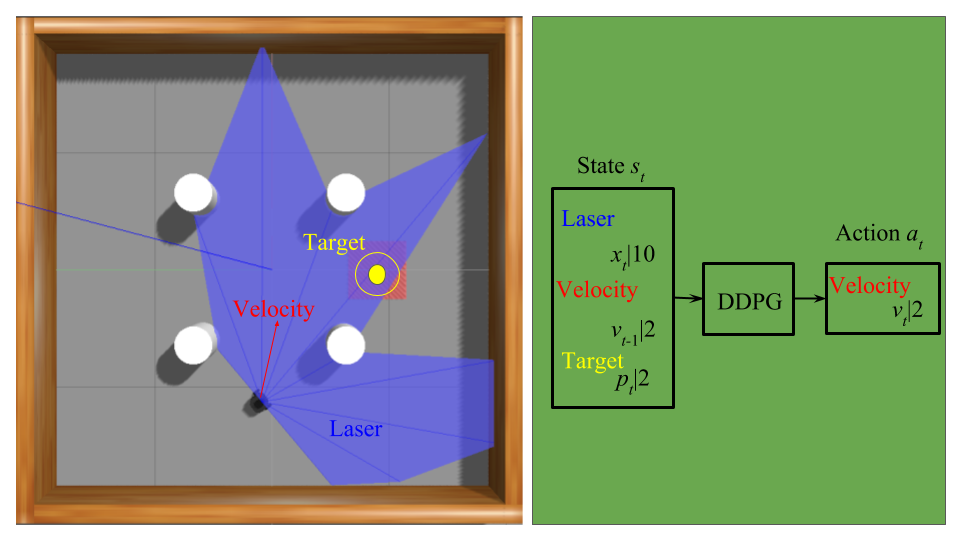
\includegraphics[width=\columnwidth]{images/mapless_en.png}}
\caption{System definition.}
\label{fig:mapless}
\end{figure}

This work is divided in seven sections.
After a brief introduction in the first section of the Deep-RL on the mobile robot navigation, the second section describes the work of authors on the field that inspired this research, the third section gives a background about the technique used, the fourth section makes an introduction of the tools used for the project, the fifth section summarizes the methods so that the robot can get to a target, the sixth section presents the results obtained on the Gazebo environments, the seventh section makes the discussion on the results and applications of Deep-RL.


% The artificial intelligence has been on a great rising on the last decades. This can be attributed for the improving of the hardware on the actual computers. The 

% % no \IEEEPARstart
% This demo file is intended to serve as a ``starter file''
% for IEEE conference papers produced under \LaTeX\ using
% IEEEtran.cls version 1.8b and later.
% % You must have at least 2 lines in the paragraph with the drop letter
% % (should never be an issue)
% I wish you the best of success.

% \hfill mds
 
% \hfill August 26, 2015

% \subsection{Related Works}
% Subsection text here.


% \subsubsection{Subsubsection Heading Here}
% Subsubsection text here.

\section{Related Works}

Deep-RL has been previously applied on robotic tasks, among this applications we can refer to the work of \cite{kober2013reinforcement}.
Which is a survey of different works of this techniques applied to robotics.
Mnih \textit{et al.} \cite{mnih2013playing} utilized a convolution neural network to estimate a value function for future rewards on the Atari games, this strategy was called deep Q-network (DQN) \cite{mnih2013playing}, \cite{hausknecht2015deep}, \cite{van2016deep}.
The DQN can only be used in a task with a discrete action.
To extend it to a continuous control, Lillicrap \textit{et al.} \cite{lillicrap2015continuous} proposed a deep deterministic policy gradients (DDPG).
That became the basement for the application of Deep-RL in mobile robot navigation.
Tai \textit{et al.} \cite{tai2017virtual} created a mapless motion planner for a mobile robot by taking the sparse 10-dimensional range findings and the target position with respect to the mobile robot coordinate frame as inputs and the continuous steering commands as output, but firstly being proposed as discrete steering commands on \cite{tai2016towards}. It was shown that, with the asynchronous Deep-RL method, a mapless motion planner can be trained and complete the task to get to a determined target. 

Zhu \textit{et al.} \cite{zhu2017target} proposed another model to apply the Deep-RL to the task of driving a mobile robot.
The model created took the current observation of states and the image of the target as input and generated an action in a 3D environment as the output.

An activity that can be very challenging in robotics is to navigate a vehicle safely and efficiently in pedestrian-rich environments. Chen \textit{et al.} \cite{chen2017socially} elaborated a Deep-RL model that can quantify what \textit{to} do and \textit{not to} do on the precise mechanism of human  navigation.
This work develops a time-efficient navigation policy that respects common social norms.
Creating a method able to control a mobile robot moving at human walking speed in an environment with many pedestrians.

\section{Theoretical Background}

\subsection{Deep Reinforcement Learning}

The goal in deep reinforcement learning is to control an agent attempting to maximize a reward function. 
The deep Q-network (DQN) algorithm \cite{mnih2013playing} was capable of human level performance on many Atari video games by estimating the actions of an agent.
However, while DQN could solve problems on complex observation spaces, it only can handle discrete action spaces. 
It is noticeable that many tasks, on the robotic control, have continuous action spaces. 
So DQN cannot be applied to continuous domains and it is necessary to use another algorithm that can handle this type of problems.

The deep deterministic policy gradients (DDPG) algorithm consists of an actor-critic method that uses approximation functions that can learn continuous action space policies. The algorithm makes use of a neural network for the actor network and other for the critic network. These two networks computes the action prediction  for the current state and generates a temporal-difference error signal for each time step. The input of the actor network is the current state, and the output is a real value representing an action chosen for a continuous action space. The output of the critic is simply the estimated Q-value of the current state and the action given by the actor.

The biggest challenge of learning in continuous action space is exploration.
To confront this challenge is needed to construct a exploration policy $\mu'$ by adding a noise sampled from a noise process $\mathcal{N}$ to the actor network policy, defined as:
\begin{equation}
\mu' = \mu(s_t) + \mathcal{N}
\end{equation}
where $\mathcal{N}$ can be chosen in a way to suit the environment.
Being the Ornstein-Uhlenbeck process \cite{uhlenbeck1930theory} the most used to generate temporally correlated exploration efficiency in physical control problems.

In general, to train and evaluate a policy function coming out of the actor network and a value function coming out of the critic network, with thousands of simulated trajectories temporally correlated, leads to the introduction of huge amounts of variance in the approximation of a true Q-function.
It is suggested to use a replay memory to store the experiences of the agent during training \cite{schaul2015prioritized}.
This means, saving the states, actions, rewards and new states that the agent explored during the episode.
And then, randomly sampling experiences to use  for learning in order to break the temporal correlations within different training episodes.

The replay of experiences allows the intelligent agent to learn from recent memories, increasing  the learning speed and breaking undesirable temporal correlations.
Even with a short memory it is possible to see a substantial improvement in the agent performance.
Despite the application of a replay memory slows the agent learning, a better performance is achieved.

Without counting the replay memory used, it is needed to make a target network to generate targets for the temporal-difference error that can regulate the learning and improve stability.
The target network contains a copy of the actor and critic, however, with ``soft" updates.
This means that the target network do not copy directly the weights of the actor and critic network.
The weights, represented by $\theta$, of the target network are then updated by:
\begin{equation}
    \theta' \leftarrow \tau\theta + (1-\tau)\theta
\end{equation}
with $\tau \ll 1$. 
Where the target is represented by the apostrophe.
So the target values of the network change slowly and allows an improvement in the stability of the learning.


\section{Experimental Setup}

For the analysis of a DDPG network was used the programming language Python \cite{ascher1999learning}. 
The Python language has as priority the legibility of the code under speed. 
The vast library and frameworks provided by Python makes it an exquisite tool for machine learning and data analysis purposes.

\subsection{ROS}

The robot operations system (ROS) is a flexible framework to write software for robots.
ROS \cite{pyo2015ros} is a collection of tools, and libraries.
ROS provides operational system's standard services, like hardware's abstraction, device low level control, messages between processes and package management. 
The set of ROS processes in execution are represented by graphs architecture where the processing is performed on nodes that receive and send messages as sensors, control, state, planning, actuator and others.

Despite the importance of low latency on the robots control, ROS is not a real-time operational system, although it is possible to integrate ROS with real-time code. This lack of real-time system is being addressed on the development of ROS 2.0.

\subsection{TurtleBot}

TurtleBot is a ROS standard platform robot, and there are 3 version of the series. TurtleBots are affordable and programmable mobile robots for use in education, research, hobby, and product prototyping.
The third version was used on this project, shown in Fig. \ref{fig:turtlebot3}.

\begin{figure}[htbp]
\centerline{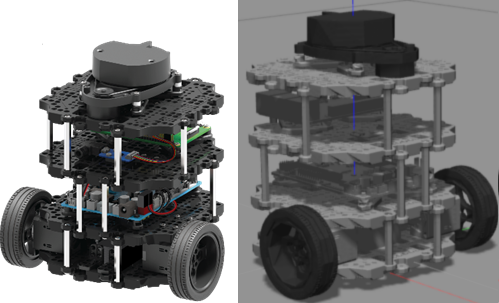
\includegraphics[width=\columnwidth]{images/burger.png}}
\caption{Real and simulated TurtleBot3 Burger in Gazebo.}
\label{fig:turtlebot3}
\end{figure}

The TurtleBot3 Burger uses 2 DYNAMIXEL motord series XL, for the object detection the TurtleBot3 utilize a 360 degree sensor laser LiDAR, and it has an IMU sensor for the odometry calculations.
All the control is made by the open source controller board OpenCR1.0 and Raspberry Pi 3 microprocessor.
% The Table \ref{tab1} shows all hardware specification of the TurtleBot3 version Burger.


% \begin{table}[htbp]
% \caption{Hardware Specication of the TurtleBot3 Burger}
% \begin{center}
% \begin{tabular}{|c|c|}
% \hline
% \textbf{Items}&\textbf{Specification} \\
% \hline
% Maximum translational velocity & 0.22 m/s \\
% \hline
% Maximum rotational velocity    & 2.84 rad/s (162.72 deg/s) \\
% \hline
% Maximum payload                & 15kg \\ 
% \hline
% Size (L x W x H)               & 138mm x 178mm x 192mm \\
% \hline
% Weight                         & 1kg \\
% \hline
% Threshold of climbing          & 10 mm or lower \\
% \hline
% Expected operating time        & 2h 30m \\
% \hline
% Expected charging time         & 2h 30m \\
% \hline
% SBC (Single Board Computers)   & Raspberry Pi 3 Model B and B+ \\
% \hline
% Actuator                       & DYNAMIXEL XL430-W250 \\
% \hline
% LDS(Laser Distance Sensor)     & 360 Laser Distance Sensor LDS-01 \\
% \hline
% IMU                            & \begin{tabular}[c]{@{}c@{}}Gyroscope 3 Axis\\ Accelerometer 3 Axis\\ Magnetometer 3 Axis\end{tabular} \\
% \hline
% Battery                        & \begin{tabular}[c]{@{}c@{}}Lithium polymer \\ 11.1V 1800mAh / 19.98Wh 5C \\ \end{tabular} \\
% \hline

% \end{tabular}
% \label{tab1}
% \end{center}
% \end{table}

\subsection{Gazebo}

Robot simulation is an essential tool on all roboticist's toolbox.
A good simulator makes possible to test algorithms quickly, to design robots, and to train systems with artificial intelligence using realistic scenarios.
With Gazebo \cite{fairchild2016ros} is possible to simulate these environments easily and with the advantage of having an active community.
This makes Gazebo a great tool on the area of robotic simulation.


\section{Methodology}

The intention of this work is to create a mobile robot that can plan its movements without any map knowledge on the environment. Its translation function is defined as:
\begin{equation}
v_t = f(x_t, p_t, v_{t-1})
\end{equation}
where $x_t$ is the observation from the raw sensor information, $p_t$ is the relative position of the target, and $v_{t-1}$ is the velocity of the mobile robot in the last time step.
All variables specified, previously, can be defined as the current state $s_t$ of the mobile robot.
With this model it is possible to get the actions that the robot will make, given its current state.
However, it is needed to ensure a minimum reading frequency of the input data to control the movement of the robot because if the robot get a slow read frequency of the inputs it cannot react to an obstacle in the trajectory to a target. In this way, the robot can react to new states quickly.
This methods was first explored by Tai \textit{et al.} \cite{tai2017virtual}.

\subsection{Network Structure}

Once the system of state and actions has been defined, it is possible to create a DDPG network capable of resolving the problem.
The DDPG network has 14 inputs as presented in Fig. \ref{fig:entradaESaida}, in which 10 corresponds to the laser range findings, 2 corresponds to the linear and angular velocity, and the other 2 corresponds to the relative position and angle of the mobile robot to the target.
The sample of the laser range findings are between $-90$ and $90$ degrees in relation to the robot. The output of the network is the action of linear and angular velocity that will be applied on the mobile robot.

\begin{figure}[htbp]
\centerline{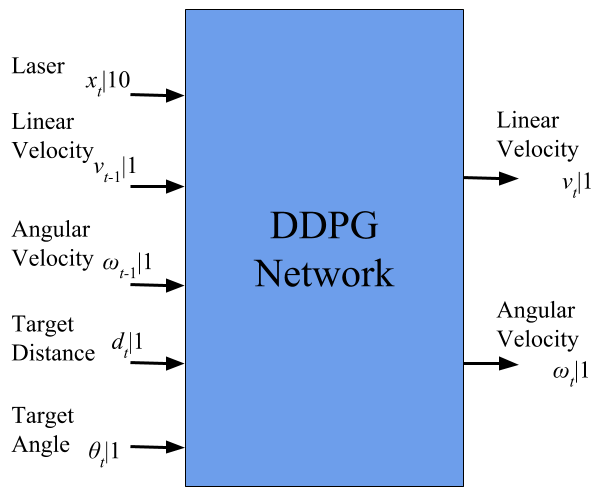
\includegraphics[width=\columnwidth]{images/o_and_i.png}}
\caption{DDPG network inputs and outputs.}
\label{fig:entradaESaida}
\end{figure}

The network structure of the DDPG is shown in Fig \ref{fig:projetointegrador}. 
The actor-network has as input the current state of the mobile robot followed by 3 fully-connected neural networks layers with 512 nodes.
This input of the networks is transformed on the linear and angular velocity that will be the commands sent to the motor of the mobile robot. 
The angular velocity range is constrained between $(-1,1)$ and the hyperbolic tangent function $(tanh)$ is used as activation function.
For the linear angular range, that it is constrained between $(0,1)$, the sigmoid function was used.
As there is no laser readings in the back of robot, the backward move is not necessary.
The output actions are then multiplied with two hyperparameters to decide the final linear and angular velocity executed by the mobile robot.
For this, it was used as maximum linear velocity $0.22$ $m/s$ and maximum angular velocity $1$ $rad/s$ on the TurtleBot3 robot version Burger.


\begin{figure}[htbp]
\centerline{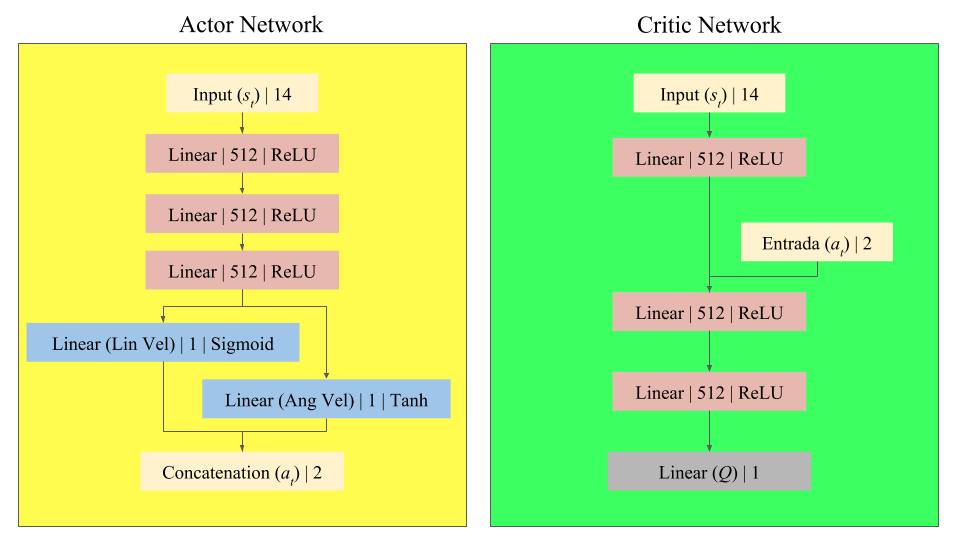
\includegraphics[width=\columnwidth]{images/projeto_integrador_en.png}}
\caption{DDPG network structure model.}
\label{fig:projetointegrador}
\end{figure}

In the critic-network, the Q-value of the current state and action are predicted.
Using only 3 fully-connected neural networks layers to process the input state.
Where the action, output of the actor-networks, is concatenated on the second neural network layer.
The Q-value is activated through a linear activation function:
\begin{equation}
y = kx +b
\end{equation}
where $x$ is the input of the last layer, $y$ is the predicted Q-value, and $k$ and $b$ are the trained weights and bias of this layer, respectively.

\subsection{Simulation Environments}

There were used three environments for the simulations. The first environment is  shown in Fig. \ref{fig:environments}(a), the environment represents a free area for the robot to move.
The walls of this environment are the only things where the robot can collide.
If the mobile robot collide with the wall or any obstacle, a negative reward is given for this action and the current episode stops.

\begin{figure}[htbp]
\centerline{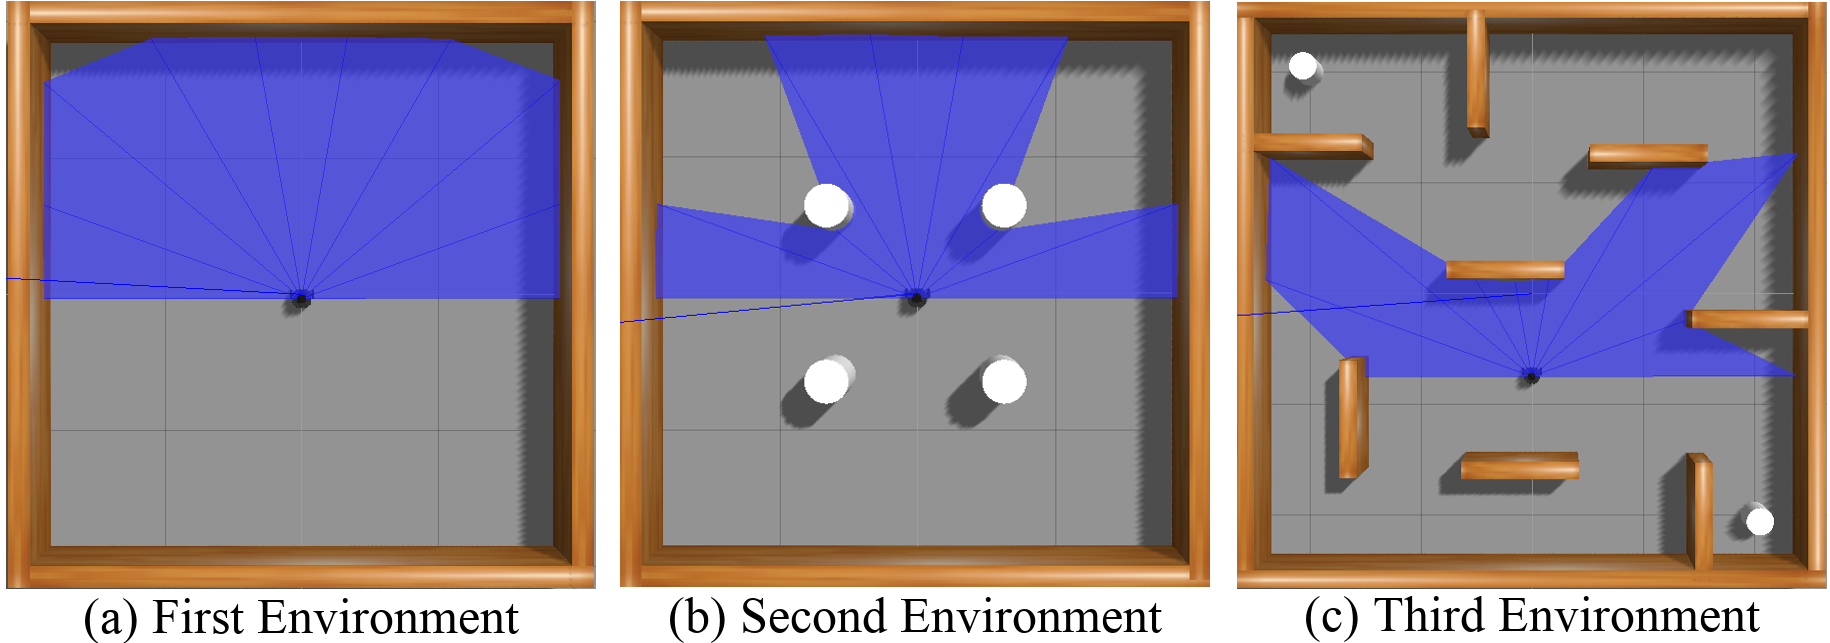
\includegraphics[width=\columnwidth]{images/environments1.png}}
\caption{Training environments used on Gazebo simulation.}
\label{fig:environments}
\end{figure}

The second environment is shown in Fig. \ref{fig:environments}(b) and has 4 fixed obstacles.
It means that this environment is more complex in a way that the intelligent agent have to make a better strategy to not collide.

The third environment, shown in Fig. \ref{fig:environments}(c), is more complex than the previous environments.  
The number of walls and the mobile obstacles, represented by the white blocks, makes the environment more dynamical, approaching it to a real-world environment.

\subsection{Reward Function}

Once the environment have been defined it is possible to simulate a controlled mobile robot for a navigation task.
Now it is necessary to define the reward and penalty system to the Deep-RL network.
Remembering that the rewards and penalties are attributed numbers passed to the intelligent agent.
So, the network will make a feedforward and backpropation step in order to learn the hyperparameters.

There are four different conditions for the reward system that presented better results for the problem's resolution and are the following:
\begin{equation}
r (s_t, a_t) = 
\begin{cases}
r_{arrive} \ \textrm{if} \ d_t < c_d
\\
r_{collide} \ \textrm{if}\ min_x < c_o
\\
c_{r1}(d_{t-1} - d_t) \ \textrm{if} \ (d_{t-1} - d_t) > 0
\\
c_{r2} \ \textrm{if} \ (d_{t-1} - d_t) \leq 0
\end{cases}
\end{equation}

If the robot gets to the target through threshold checking $c_d$, a positive reward $(r_{arrive})$ is given, but if the robot collides with an obstacle through a minimum range readings checking, a negative reward $(r_{collide})$ is given.
Both conditions are sufficient to end the training episode.
Otherwise, the reward is based on the distance difference from the target compared to the last time step $(d_{t-1} - d_t)$. 
If this difference is positive the reward given is the distance traveled multiplied by the hyperparameter $(c_{r1})$, and if the distance is negative is used the hyperparameter $(c_{r2})$.
This motivates the mobile robot to get closer to the target position and encourages it to avoid the obstacles in the environment.




\section{Results}

This section deals with the presentation and discussion of results.
The collected data are related to the obtained reward from the artificial neural network of the project.
With these data is possible to see what is the learning degree of the agent in the environment because the gained reward is intrinsically attached to the performance of the agent on the environment that it must go.
All the training environments were arranged by ROBOTIS, however, some alterations were done on the source code of the Gazebo simulation in order for the simulated mobile robot to use the reward system defined on this paper.

A mobile robot with a DDPG network was trained in order to make the experiments in the environments presented on Fig. \ref{fig:environments}, where the goal of the mobile robot is to get to the target.
For the first test was used the first environment that shows, in Fig. \ref{fig:amb1target}, a sequence of frames of the robot and the target. We can observe how the robot start in an initial position distant from the target, navigating in order to reach the target.

\begin{figure}[htbp]
\centerline{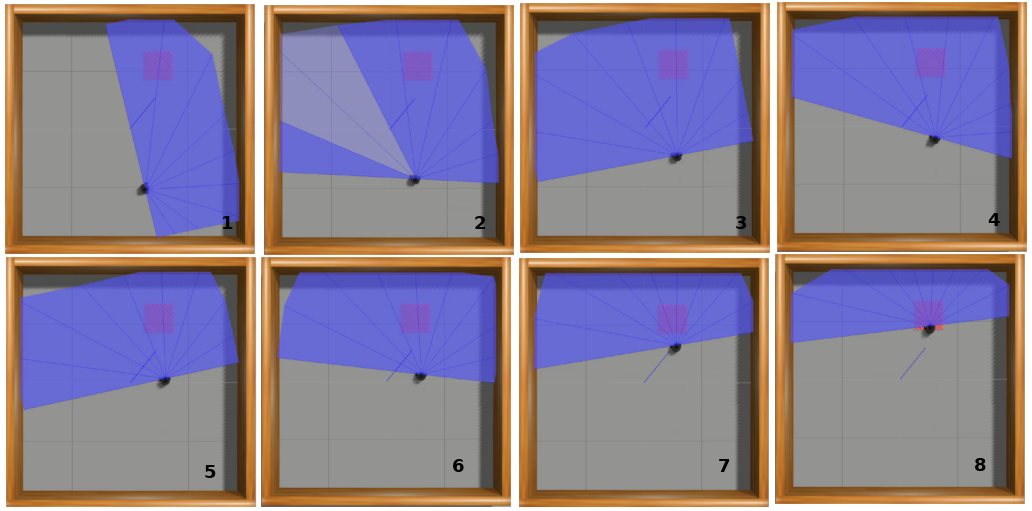
\includegraphics[width=\columnwidth]{images/amb1target.png}}
\caption{Images sequence in the first environment.}
\label{fig:amb1target}
\end{figure}

The training results of the reward function of the first environment are shown in Fig. \ref{fig:stage_1}.
On the first episodes can be noticed a negative reward, this happens because the algorithm started and it was still learning. 
This reward by episode means that the robot is trying to maximize the reward to complete the task. 
It is observed in the episode 400 a fall. 
This is a probable correction on some maximized parameters of the network and it resulted in a low reward.
Results like this means that the network has a continuous learning trying to correct itself. 

\begin{figure}[htbp]
\centerline{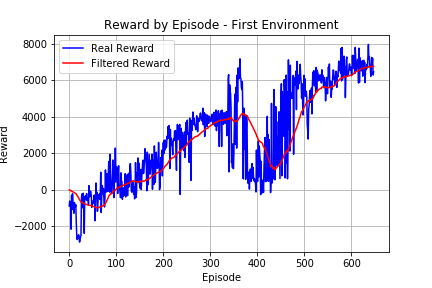
\includegraphics[width=\columnwidth]{images/stage_1.png}}
\caption{Rewards of the first environment.}
\label{fig:stage_1}
\end{figure}

In Fig. \ref{fig:stage_1} the $x$ axis represents the past episodes on the simulation, an episode is defined when the mobile robot arrives to the target in the map or collides with some obstacle. 
The $y$ axis in Fig. \ref{fig:stage_1} represents the total value of the reward that the robot received on the episode.
The reward, with the blue color, has a great variance, it was decided to use a moving average filter for better visualization of the results.

After the mobile robot has been trained on the first environment, the experiment was done in the second environment and tested. It is shown in Fig. \ref{fig:amb2target} a sequence of the actions made by the TurtleBot from an initial position until it could arrive to the target after the training episodes.

\begin{figure}[htbp]
\centerline{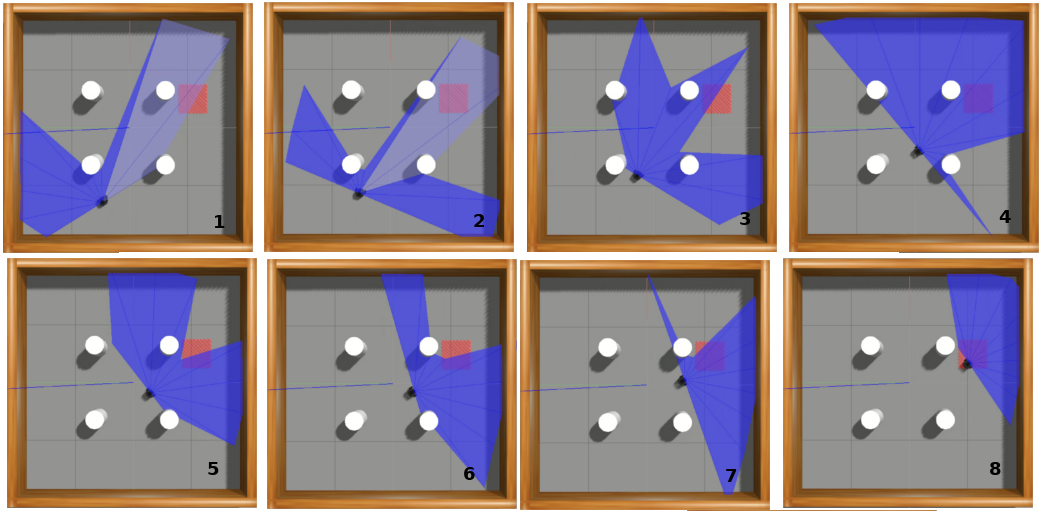
\includegraphics[width=\columnwidth]{images/amb2target.png}}
\caption{Images sequence in the second environment.}
\label{fig:amb2target}
\end{figure}

The reward function results of the training process for the second environment are shown in Fig. \ref{fig:stage_2}.
Comparing this results with the last environment, we can observe that it needed more episodes so the robot could present good results.
It is noticed that with a more complex environment, exists the possibility that an agent could take a longer time to get a good performance.

\begin{figure}[htbp]
\centerline{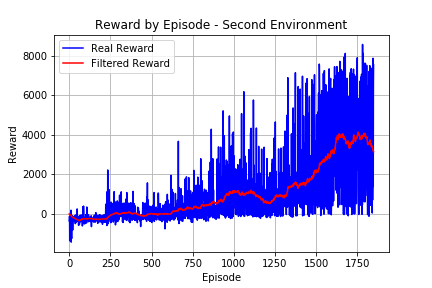
\includegraphics[width=\columnwidth]{images/stage_2.png}}
\caption{Rewards of the second environment.}
\label{fig:stage_2}
\end{figure}

For the final test and the sequence of the actions made by the TurtleBot to arrive to the target after the training process it was used the third environment.  A sequence of the actions made by the TurtleBot to arrive to the target after the training episodes are shown in Fig. \ref{fig:amb3target}.

\begin{figure}[htbp]
\centerline{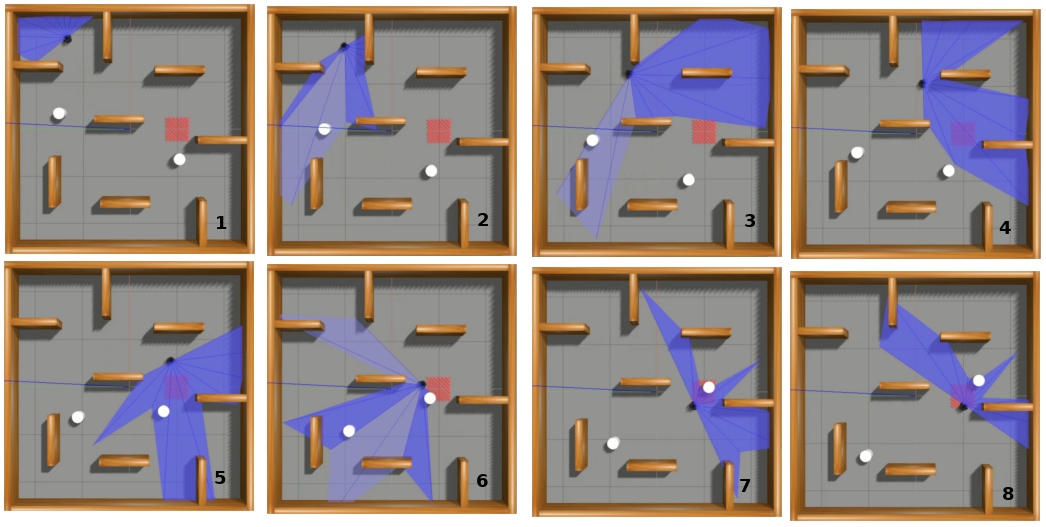
\includegraphics[width=\columnwidth]{images/amb3target.png}}
\caption{Images sequence in the third environment.}
\label{fig:amb3target}
\end{figure}

The results of the reward function of the last training environment is shown in Fig. \ref{fig:stage_4}.
On this environment, due to the high complexity, it was necessary a higher number of training episodes.
If compared the reward function with the previous Fig. \ref{fig:stage_1} and Fig. \ref{fig:stage_2}, it is possible to notice an average reward bellow two thousand.
This happens because to reach the target, which has the highest reward possible on comparison with the others, it is necessary that the agent could execute actions that do not generate too many points, however, that still makes it to arrive to the target.
Nevertheless, it was noticed by simulating the trained robot some actions that caused it to collide.
Many of these collisions were due to the moving dynamic obstacle close to the target.
This resulted in the agent making the decision of that mobile robot would collide or would try to avoid the obstacle.
The occurred behavior may have been caused because of the system created.
In order to resolve these actions, probably, it would be necessary to create a reward system that could bypass the error of the network.

\begin{figure}[htbp]
\centerline{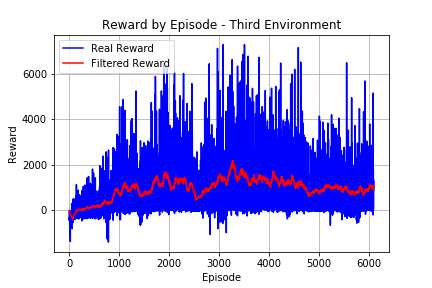
\includegraphics[width=\columnwidth]{images/stage_4.png}}
\caption{Rewards of the third environment.}
\label{fig:stage_4}
\end{figure}

% An example of a floating figure using the graphicx package.
% Note that \label must occur AFTER (or within) \caption.
% For figures, \caption should occur after the \includegraphics.
% Note that IEEEtran v1.7 and later has special internal code that
% is designed to preserve the operation of \label within \caption
% even when the captionsoff option is in effect. However, because
% of issues like this, it may be the safest practice to put all your
% \label just after \caption rather than within \caption{}.
%
% Reminder: the "draftcls" or "draftclsnofoot", not "draft", class
% option should be used if it is desired that the figures are to be
% displayed while in draft mode.
%
%\begin{figure}[!t]
%\centering
%\includegraphics[width=2.5in]{myfigure}
% where an .eps filename suffix will be assumed under latex, 
% and a .pdf suffix will be assumed for pdflatex; or what has been declared
% via \DeclareGraphicsExtensions.
%\caption{Simulation results for the network.}
%\label{fig_sim}
%\end{figure}

% Note that the IEEE typically puts floats only at the top, even when this
% results in a large percentage of a column being occupied by floats.


% An example of a double column floating figure using two subfigures.
% (The subfig.sty package must be loaded for this to work.)
% The subfigure \label commands are set within each subfloat command,
% and the \label for the overall figure must come after \caption.
% \hfil is used as a separator to get equal spacing.
% Watch out that the combined width of all the subfigures on a 
% line do not exceed the text width or a line break will occur.
%
%\begin{figure*}[!t]
%\centering
%\subfloat[Case I]{\includegraphics[width=2.5in]{box}%
%\label{fig_first_case}}
%\hfil
%\subfloat[Case II]{\includegraphics[width=2.5in]{box}%
%\label{fig_second_case}}
%\caption{Simulation results for the network.}
%\label{fig_sim}
%\end{figure*}
%
% Note that often IEEE papers with subfigures do not employ subfigure
% captions (using the optional argument to \subfloat[]), but instead will
% reference/describe all of them (a), (b), etc., within the main caption.
% Be aware that for subfig.sty to generate the (a), (b), etc., subfigure
% labels, the optional argument to \subfloat must be present. If a
% subcaption is not desired, just leave its contents blank,
% e.g., \subfloat[].


% An example of a floating table. Note that, for IEEE style tables, the
% \caption command should come BEFORE the table and, given that table
% captions serve much like titles, are usually capitalized except for words
% such as a, an, and, as, at, but, by, for, in, nor, of, on, or, the, to
% and up, which are usually not capitalized unless they are the first or
% last word of the caption. Table text will default to \footnotesize as
% the IEEE normally uses this smaller font for tables.
% The \label must come after \caption as always.
%
%\begin{table}[!t]
%% increase table row spacing, adjust to taste
%\renewcommand{\arraystretch}{1.3}
% if using array.sty, it might be a good idea to tweak the value of
% \extrarowheight as needed to properly center the text within the cells
%\caption{An Example of a Table}
%\label{table_example}
%\centering
%% Some packages, such as MDW tools, offer better commands for making tables
%% than the plain LaTeX2e tabular which is used here.
%\begin{tabular}{|c||c|}
%\hline
%One & Two\\
%\hline
%Three & Four\\
%\hline
%\end{tabular}
%\end{table}


% Note that the IEEE does not put floats in the very first column
% - or typically anywhere on the first page for that matter. Also,
% in-text middle ("here") positioning is typically not used, but it
% is allowed and encouraged for Computer Society conferences (but
% not Computer Society journals). Most IEEE journals/conferences use
% top floats exclusively. 
% Note that, LaTeX2e, unlike IEEE journals/conferences, places
% footnotes above bottom floats. This can be corrected via the
% \fnbelowfloat command of the stfloats package.



\section{Conclusion}

In this paper was developed a neural network, DDPG, to be used on navigation of a mobile robot through continuous control in a virtual environment.
Thus achieving a deep reinforcement learning network structure able to solve the problem of robot navigation.
It was proposed as a task that the robot could reach a target position in different simulated environments and it created a reward function so that the DDPG network could give as results, the linear and angular velocity for the robot. All the network structure created was applied on the Gazebo simulation environments with success.

With the training results obtained on the simulation environments, it was analyzed the performance of the intelligent agent algorithm in the task of avoiding obstacles and getting to the final goal. 
On the three environments proposed, the algorithm had a good performance, however, in the last environment it was observed that sometimes even after many training episodes the mobile robot would still collide with some obstacle.

It is possible to conclude that DDPG networks are suitable for the development of applications that need a continuous control on the robotics.
The Deep-RL networks can produce excellent results if the reward system is well-made for the problem that it wants to solve.
It was proved that intelligent agents can move around in a complex simulated environment without any previous knowledge of the environment.
The network based on deep deterministic policy gradients can provide means of unifying the machine learning for the control of robotic systems.
This technique can be applied in function as manipulation of robotic arms, pendulums, games among others.
As future works, it is intended to use the deep reinforcement learning technique for the navigation of the TurtleBot3 Burger robot in a real environment, thus, being able to validate the training in a simulated environment in a real environment.




% conference papers do not normally have an appendix


% use section* for acknowledgment
% \section*{Acknowledgment}


% The authors would like to thank...





% trigger a \newpage just before the given reference
% number - used to balance the columns on the last page
% adjust value as needed - may need to be readjusted if
% the document is modified later
%\IEEEtriggeratref{8}
% The "triggered" command can be changed if desired:
%\IEEEtriggercmd{\enlargethispage{-5in}}

% references section

% can use a bibliography generated by BibTeX as a .bbl file
% BibTeX documentation can be easily obtained at:
% http://mirror.ctan.org/biblio/bibtex/contrib/doc/
% The IEEEtran BibTeX style support page is at:
% http://www.michaelshell.org/tex/ieeetran/bibtex/
%\bibliographystyle{IEEEtran}
% argument is your BibTeX string definitions and bibliography database(s)
%\bibliography{IEEEabrv,../bib/paper}
%
% <OR> manually copy in the resultant .bbl file
% set second argument of \begin to the number of references
% (used to reserve space for the reference number labels box)

% \begin{thebibliography}{1}

% \bibitem{IEEEhowto:kopka}
% H. Kopka and P. W. Daly, \emph{A Guide to \LaTeX}, 3rd~ed.\hskip 1em plus
%   0.5em minus 0.4em\relax Harlow, England: Addison-Wesley, 1999.

% \end{thebibliography}

\bibliographystyle{IEEEtran}
\bibliography{IEEEabrv,bibliography}


% that's all folks
\end{document}


